\chapter{\label{cha:sts_siamese_neural_networks}Siamese Neural Networks for STS}

A \textit{Siamese Neural Network} refers to a class of neural network architecture that contains two or more identical subnetworks. This is usually employed in applications that require comparisons between two or more inputs (signature verification, image similarity etc.). The network can take two or more inputs at the same time and they will be processed by different subnetworks simultaneously. The subnetworks have the same configuration with identical parameters and weights. The training process is mirrored across all of the subnetworks, meaning that the parameters remain constant across all of the subnetworks. Each subnetwork contains a traditional perceptron model such as LSTM, CNN etc. The neural network compares the outputs of the two subnetworks through a distance metric such as cosine distance, and the error is propagated back \autocite{Mueller_Thyagarajan_2016}. In the testing phase, the neural network predicts whether the two inputs are different through this similarity measure \autocite{neculoiu-etal-2016-learning}. 

Siamese neural networks have been employed in many applications in different areas such as signal processing \autocite{thiolliere2015hybrid, 8461524, 8268960, 8453811, 10.1007/978-3-319-66429-3_11, 8064706, 8268994, Zeghidour2016}, biology \autocite{10.1093/bioinformatics/bty887, Szubert2019}, chemistry and pharmacology \autocite{10.1093/bioinformatics/btz411}, geometry \autocite{10.1093/jcde/qwaa003}, computer vision  \autocite{6797067,1467314,rs10020355,21be1428c6a44fb7a32d49ba83126bcb,6976727,6636646,Taigman_2014_CVPR,7163112,8269987,HANIF201954}, physics \autocite{Zou18, DEBAETS2019645}, robotics \autocite{Utkin2017, 7970671, 8461044}, video processing \autocite{AAAI1816790, 8036238, Liu2018, 8587153} etc. They have also been used in NLP tasks \autocite{10.5555/2018936.2018965,10.1145/3209978.3210144,Gonzalez2019} including STS \autocite{das-etal-2016-together, neculoiu-etal-2016-learning, Mueller_Thyagarajan_2016}. In fact, the best result from the SICK dataset \autocite{marelli-etal-2014-semeval} was provided by a Siamese neural network \autocite{Mueller_Thyagarajan_2016} which shows that state-of-the-art in STS are Siamese neural networks. 

In addition to providing state-of-the-art results in STS, there are additional advantages of using Siamese neural networks. As previously mentioned, in Siamese neural networks the weights are shared across subnetworks resulting in fewer parameters to train, this in turn means that less training data is required and there is a lower likelihood of overfitting  \autocite{ranasinghe-etal-2019-semantic}. Given the amount of human labour required to produce datasets for STS, Siamese neural networks can provide an ideal solution. Another advantage is that when trained on a STS task the Siamese neural network architecture can be adapted as a sentence encoder. The output vector of the subnetwork is a semantically rich vector representation of the input sentence \autocite{Mueller_Thyagarajan_2016}. These advantages have motivated us to further explore Siamese neural network architectures in STS. 


We address four research questions in this chapter:

\textbf{RQ1:} Can an existing state-of-the-art Siamese neural network architecture be modified to provide better STS results?

\textbf{RQ2:} Can the method be further improved with transfer learning and data augmentation techniques?

\textbf{RQ3:} Can the proposed Siamese neural network be easily adapted for different languages?

\textbf{RQ4:} How well does the proposed Siamese neural network perform in a different domain? 


The main contributions of this chapter are as follows.

\begin{enumerate}
	\item We propose a GRU (Gated Recurrent Unit) based Siamese neural network that outperformed the state-of-the-art LSTM based Siamese neural network in small STS datasets. 
	
	\item We propose an LSTM (Long Short Term Memory) and self-attention based Siamese neural network that outperformed the state-of-the-art LSTM based Siamese neural network in large STS datasets.
	
	\item We propose further enhancements to the architecture using transfer learning and data augmentation.  
	
	\item We evaluate how well the proposed Siamese neural network architecture performs in different languages and domains. 
	
	\item The code and the pre-trained models are publicly available to the community\footnote{The public GitHub repository is available on \url{https://github.com/tharindudr/Siamese-recurrent-rrchitectures}}.
\end{enumerate}


The rest of this chapter is organised as follows. Section \ref{sec:siamese_related} describes the existing research done on Siamese neural networks. Section \ref{sec:siamese_method} discusses the methodology and the experiments undertaken with three English STS datasets. Sections \ref{sec:siamese_transfer} and \ref{sec:siamese_aug} provide more experiments which improve the results. Experiments conducted with other languages and domains are shown in Sections \ref{sec:siamese_languages} and \ref{sec:siamese_domains}. The chapter finishes with conclusions and ideas for future research directions in Siamese neural networks. 

\section{Related Work}
\label{sec:siamese_related}

The Siamese neural networks are prevalent in the machine learning community. The first appearance of Siamese neural networks date back to 1993 when they were first introduced by \textcite{doi:10.1142/S0218001493000339} to detect forged signatures. By comparing two handwritten signatures, this Siamese neural network could predict if the two signatures were both original or if one was a forgery. Preceding this, \textcite{6797067} introduced a similar artificial neural network able to recognise fingerprints, though by a different name. 

Siamese neural networks have been employed for various uses since these initial applications. In the audio and speech signal processing field, \textcite{thiolliere2015hybrid} merged a dynamic-time warping based spoken term discovery (STD) system with a Siamese deep neural network for the automatic discovery of linguistic units from raw speech. \textcite{8461524} used a Siamese model to detect all semantically similar audio clips from an input audio recording, and \textcite{8268960} employed a Siamese model to recognise Arabic dialects from the Arabic speech content found in media broadcasts. In biology, \textcite{10.1093/bioinformatics/bty887} implemented a Siamese neural network to compare DNA sequences and recently \textcite{Szubert2019} presented a Siamese neural network-based technique for a visualisation and interpretation of single-cell datasets. Image analysis is the field with the highest number of applications for the Siamese neural networks. Recognising fingerprints \autocite{6797067}, similar image detection \autocite{1467314,rs10020355,21be1428c6a44fb7a32d49ba83126bcb,6976727,6636646}, face verification \autocite{Taigman_2014_CVPR}, gesture recognition \autocite{7163112}, handwriting analysis \autocite{8269987} and patch matching \autocite{HANIF201954} are some examples of them. All of these tasks involve the comparison of two or more things.

Recently, Siamese neural networks have also been employed in NLP. \textcite{10.5555/2018936.2018965} proposed similarity Learning via Siamese Neural Network (S2Net), a technique able to discriminatingly learn the concept vector representations of text words. \textcite{10.1145/3209978.3210144} used a Siamese neural network to recognise clickbaits in online media outlets. \textcite{Gonzalez2019} proposed a natural language processing application of the Siamese neural network for extractive summarisation, which means that their technique can extrapolate the most relevant sentences in a document. 

Siamese neural networks are not limited to these applications and have also been implemented in STS tasks in NLP. \textcite{das-etal-2016-together} used a CNN based Siamese neural network to detect similar questions on question and answer websites such as Yahoo Answers, Baidu, Zhidao, Quora, and Stack Overflow. \textcite{neculoiu-etal-2016-learning} employed a Siamese neural network based on Bidirectional LSTMs to identify similar job titles. The baseline we used for this chapter, MALSTM \autocite{Mueller_Thyagarajan_2016} uses LSTM based Siamese neural network to produce semantic textual similarity, and it provides the best results for the SICK dataset outperforming other STS methods such as Tree-LSTMs \autocite{tai-etal-2015-improved}. They use the exponent of the negative Manhattan distance between two outputs from the two subnetworks as the similarity function. Due to the performance, this can be considered as the state-of-the-art Siamese neural network for STS. However, this architecture leaves considerable room for variation, which we exploit in this chapter as we explain in Section \ref{sec:siamese_method}.

\section{Exploring Siamese Neural Networks for STS}
\label{sec:siamese_method}

The basic structure of the Siamese neural network architecture used in our experiments is shown in Figure \ref{fig:siamese}. It consists of an embedding layer that represents each sentence as a sequence of word vectors. This sequence of word vectors is then fed into a Recurrent Neural Network (RNN) cell, which learns a mapping from the space of variable-length sequences of 300-dimensional vectors into a 50 dimensional vector. The sole error signal backpropagated during training stems from the similarity between these 50 dimensional vectors, which can also be used as a sentence representation. Initially, the similarity function we used was based on Manhattan distance. To ensure that the prediction is between 0 and 1, we took the exponent of the negative Manhattan distance between two sentence representations. The similarity function was adapted from \textcite{Mueller_Thyagarajan_2016}. The proposed variants of our architecture are:


\begin{enumerate}
	\item LSTM - Block A in Figure \ref{fig:siamese} contains a single LSTM cell. This is the architecture suggested by \textcite{Mueller_Thyagarajan_2016} 
	
	\item Bi-directional LSTM - Block A in Figure \ref{fig:siamese} contains a single Bi-directional LSTM cell. Bi-directional LSTM tends to understand the context better than Unidirectional LSTM \autocite{650093}.
	
	\item GRU - Block A in Figure \ref{fig:siamese} contains a single GRU cell. GRUs have been shown to exhibit a better performance on smaller datasets \autocite{Chung2014EmpiricalEO}. 
	
	\item Bi-directional GRU - Block A in Figure \ref{fig:siamese} contains a single Bi-directional GRU cell. Bi-directional GRUs tend to understand the context better than Unidirectional GRUs \autocite{vukotic:hal-01351733}.
	
	\item LSTM + Attention - Block A in Figure \ref{fig:siamese} contains a single LSTM cell with self attention \autocite{NIPS2017_3f5ee243}.
	
	\item GRU + Attention - Block A in Figure \ref{fig:siamese} contains a single GRU cell with self attention \autocite{NIPS2017_3f5ee243}.
	
	\item GRU + Capsule + Flatten - Block A in Figure \ref{fig:siamese} contains a GRU followed by a capsule layer and a flatten layer. Dynamic routing used between capsules performs better than a traditional max-pooling layer \autocite{NIPS2017_2cad8fa4}.
	
\end{enumerate}

\begin{figure}[ht]
	\centering
	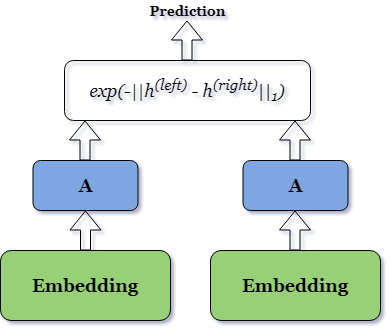
\includegraphics[scale=0.5]{figures/semantic_textual_similarity/siamese_neural_networks/siamese_architecture.png}
	\caption[Basic structure of the Siamese neural network]{Basic structure of the Siamese neural network. Unit A is changed over the architectures.}
	\label{fig:siamese}
\end{figure}


As the word embedding model, we used Word2vec embeddings \autocite{DBLP:journals/corr/abs-1301-3781} pre-trained on the Google news corpus\footnote{Pre-trained Word2vec can be downloaded from \url{https://code.google.com/archive/p/word2vec/}}. Using this model, we represented each word as a 300 length vector. For the words that do not appear in the model, we used a random vector. 
We evaluated all of the above variations in the three English STS datasets we introduced in \ref{cha:sts_introduction}; SICK, STS 2017 and QUORA. We trained the Siamese models on the training sets in these datasets and evaluated them on the testing sets. The results are shown in Table \ref{tab:sick_siamese}, Table \ref{tab:sts_siamese} and Table \ref{tab:quora_siamese} respectively.


\begin{table*}[htb]
	%\footnotesize
	\centering
	\scalebox{0.95}{
		\begin{tabular}{|l|cc|}
			\hline
			\textbf{Model} & $\bm{\rho}$   & $\bm{\tau}$     
			\\ \hline
			\textit{LSTM}                  
			& 0.802 & 0.733  \\
			\textit{Bi-LSTM}                     
			& 0.784 & 0.708   \\
			\textit{GRU}                     
			& 0.838$^{\dagger}$ & 0.780$^{\dagger}$  \\
			\textit{Bi-GRU}                     
			& 0.832 & 0.773  \\
			\textit{LSTM + Attention}                     
			& 0.827  & 0.765       \\
			\textit{GRU + Attention}                     
			& 0.818  & 0.751       \\
			\textit{GRU + Capsule + Flatten}                     
			& 0.806  & 0.733       \\
			\hline
		\end{tabular}
	}
	\caption[Results for SICK with Siamese Neural Network]{Results for SICK dataset with different variants of Siamese Neural Network. For each variant, Pearson Correlation ($\bm{\rho}$) and Spearman Correlation ($\bm{\tau}$) are reported between the predicted values and the gold labels of the test set. The best result from all the variations is marked with ${\dagger}$.}  
	\label{tab:sick_siamese}
\end{table*}


\begin{table*}[htb]
	%\footnotesize
	\centering
	\scalebox{0.95}{
		\begin{tabular}{|l|cc|}
			\hline
			\textbf{Model} & $\bm{\rho}$   & $\bm{\tau}$     
			\\ \hline
			\textit{LSTM}                  
			& 0.831 & 0.762  \\
			\textit{Bi-LSTM}                     
			& 0.784 & 0.708   \\
			\textit{GRU}                     
			& 0.853$^{\dagger}$ & 0.811$^{\dagger}$  \\
			\textit{Bi-GRU}                     
			& 0.844 & 0.804  \\
			\textit{LSTM + Attention}                     
			& 0.830  & 0.791       \\
			\textit{GRU + Attention}                     
			& 0.825  & 0.782       \\
			\textit{GRU + Capsule + Flatten}                     
			& 0.806  & 0.765       \\
			\hline
		\end{tabular}
	}
	\caption[Results for STS 2017 with Siamese Neural Network]{Results for STS 2017 dataset with different variants of Siamese Neural Network. For each variant, Pearson Correlation ($\bm{\rho}$) and Spearman Correlation ($\bm{\tau}$) are reported between the predicted values and the gold labels of the test set. The best result from all the variations is marked with ${\dagger}$. }  
	\label{tab:sts_siamese}
\end{table*}


\begin{table*}[htb]
	%\footnotesize
	\centering
	\scalebox{0.95}{
		\begin{tabular}{|l|c|}
			\hline
			\textbf{Model} & RMSE     
			\\ \hline
			\textit{LSTM}                  
			& 0.412   \\
			\textit{Bi-LSTM}                     
			& 0.402    \\
			\textit{GRU}                     
			& 0.415  \\
			\textit{Bi-GRU}                     
			& 0.408   \\
			\textit{LSTM + Attention}                     
			& 0.382$^{\dagger}$        \\
			\textit{GRU + Attention}                     
			& 0.398       \\
			\textit{GRU + Capsule + Flatten}                     
			& 0.421        \\
			\hline
		\end{tabular}
	}
	\caption[Results for QUORA with Siamese Neural Network]{Results for QUORA dataset with different variants of Siamese Neural Network. For each variant, Root Mean Squared Error (RMSE) reported between the predicted values and the gold labels of the test set. The best result from all the variations is marked with ${\dagger}$. }  
	\label{tab:quora_siamese}
\end{table*}

As can be seen in Tables \ref{tab:sick_siamese} and \ref{tab:sts_siamese}, for the SICK and STS2017 datasets, the GRU based Siamese neural network model outperformed the LSTM based Siamese neural network model, which we used as a baseline, and this provided the best result. It can be seen that complex architectures that involve Bi-directional RNNs, Attention and Capsule mechanisms did not perform well when compared to simple architectures like GRU. We can conclude that for the smaller datasets like STS 2017 and SICK, the GRU based architecture performs better because GRU has fewer parameters than LSTM \autocite{Chung2014EmpiricalEO}. With fewer parameters, the architecture does not need many training instances to optimise the weights during the training process.

However, when it comes to the big STS dataset, QUORA, the way the variants of the Siamese neural network behaves is different. As we introduced in Chapter \ref{cha:sts_introduction}, QUORA was the biggest STS dataset we experimented with, and it has 320,000 training instances. As a result, even complex architectures like RNNs with Attention get the opportunity to optimise their parameters and deliver good results. This can be seen in Table \ref{tab:quora_siamese}. For the QUORA dataset, the LSTM + Attention based Siamese neural network model outperformed the LSTM based Siamese neural network model, which we used as a baseline, and provided the best result. For bigger datasets, we can conclude that Siamese neural networks based on LSTM with Attention would outperform Siamese neural networks only with LSTMs. 

From the variants we examined, one notable observation is the poor performance of capsules in Siamese architectures. Despite providing good results in many NLP tasks such as text classification \autocite{NIPS2017_2cad8fa4,hettiarachchi-ranasinghe-2019-emoji, xia-etal-2018-zero, srivastava-etal-2018-identifying} and relation extraction \autocite{Zhang_Li_Jia_Zhao_2019, zhang-etal-2018-attention, 9095302}, the capsule-based variant failed to outperform the simple LSTM based variant even in the bigger STS dataset. This observation implies that capsule-based Siamese neural networks will not be a good fit for STS tasks.

With these findings, we answer our \textbf{RQ1} in this chapter. We have improved the state-of-the-art Siamese neural network architecture and propose a GRU based Siamese neural network architecture for the smaller STS datasets and LSTM + Attention based Siamese neural network for larger STS datasets.

\subsection{Impact of Transfer Learning}
\label{sec:siamese_transfer}
Transfer learning is a machine learning method where a model developed for a task is reused as the starting point for a model on a second task. It is a popular approach in deep learning where pre-trained models are used as the starting point for a new task. This is usually done in scenarios where there is not enough data to train a neural network, so that starting from already finetuned weights would be advantageous \autocite{pmlr-v97-houlsby19a, ruder-etal-2019-transfer}. Transfer learning has often provided good results for smaller datasets. Therefore, we explored the impact of transfer learning with Siamese neural networks in STS.

We saved the weights of the models that were trained on each STS dataset; SICK, STS 2017 and QUORA. We specifically used the two models that performed best in these datasets; Siamese neural network with GRU and the Siamese neural network with LSTM + Attention. We initiated training for each dataset, however rather than training from scratch, we used the weights of the models trained on another STS dataset. We compared these transfer learning results to the results we got from training the model from scratch. We conducted this transfer learning experiment only on the STS2017 and SICK datasets since the QUORA dataset is already large and transfer learning from a smaller dataset to a larger dataset is nonsensical.


\begin{table*}[htb]
	%\footnotesize
	\centering
	\scalebox{0.95}{
		\begin{tabular}{|l|c|c|}
			\hline
			\textbf{Start Model} & STS2017 & SICK      
			\\ \hline
			\textit{STS2017$_{GRU}$}                  
			& 0.853 & \textcolor{gray}{(+0.01)} \\
			\textit{STS2017$_{LSTM+Aten}$}                     
			& 0.830 & \textcolor{gray}{(+0.01)}  \\
			\hline
			\textit{SICK$_{GRU}$}                     
			& \textcolor{gray}{(+0.01)} & 0.838 \\
			\textit{SICK$_{LSTM+Aten}$}                     
			& \textcolor{gray}{(+0.01)} & 0.827 \\
			\hline
			\textit{QUORA$_{GRU}$}                     
			& \textcolor{gray}{(-0.02)}  &  \textcolor{gray}{(-0.02)}    \\
			\textit{QUORA$_{LSTM+Aten}$}                     
			& \textcolor{gray}{(-0.04)} &  \textcolor{gray}{(-0.04)}    \\
			\hline
		\end{tabular}
	}
	\caption[Results for transfer learning with Siamese Neural Network]{Results for transfer learning with different variants of Siamese Neural Network. For each transfer learning experiment we show the difference between with and without transfer learning. Non-grey values are the results of the experiments without transfer learning which we showed in the previous section. For ease of visualisation we only report the Pearson correlation ($\bm{\rho}$).}  
	\label{tab:transfer_siamese}
\end{table*}

As can be seen in Table \ref{tab:transfer_siamese} some of the transfer learning experiments improved the results for the STS2017 and SICK datasets with both architectures. The results improved when we performed transfer learning from STS2017 $\Rightarrow$ SICK and SICK $\Rightarrow$ STS2017. This shows that transfer learning can improve the results in Siamese neural networks. However, when we performed transfer learning from QUORA $\Rightarrow$ STS2017 and QUORA $\Rightarrow$ SICK, the results did not improve. In fact, they decrease, despite QUORA being the largest STS dataset we experimented with. This finding is somewhat controversial as the general belief in the community is that transfer learning from a larger dataset will improve the result. In this case, we believe that this happened because the QUORA dataset is very different to the other two datasets, as discussed in Chapter \ref{cha:sts_introduction}. Despite QUORA having a large number of training instances, when performing transfer learning, the neural network finds it difficult to optimise the weights for STS2017 and SICK as they were already optimised for a very different dataset; QUORA. This leads to a decrease in the results. On the other hand, transfer learning between STS2017 and SICK improved the results for both datasets since they are similar in nature, as we discussed in Chapter \ref{cha:sts_introduction}. 

Therefore, we can conclude that transfer learning can improve the results for Siamese neural networks in STS. However, the transfer learning dataset should be picked carefully taking the similarity of the two datasets into consideration, rather than only considering the size of the dataset.


\subsection{Impact of Data Augmentation}
\label{sec:siamese_aug}
As we observed earlier, the neural networks perform better when there are large number of training instances. Therefore, many approaches have been taken to increase the number of training instances. Usually, this has resulted in better performance with neural networks \autocite{wei-zou-2019-eda}. Therefore, we examined the impact of data augmentation on the Siamese neural network architectures proposed previously. We only conducted this experiment with the STS 2017 and SICK datasets as QUORA already has a large number of training instances.

We employed thesaurus-based augmentation in which 10,000 additional training examples are generated by replacing random words with one of their synonyms from Wordnet \autocite{10.1145/219717.219748}. A similar approach has also been successfully adapted by \textcite{Mueller_Thyagarajan_2016}, and \textcite{10.5555/2969239.2969312}.  We specifically used the two models that performed best with the bigger dataset and smaller dataset; Siamese neural network with GRU and Siamese neural network with LSTM + Attention. Since using transfer learning improved the results in the previous experiment, we trained the augmented training set on the transferred models; models trained on STS2017 for the SICK experiments and models trained on SICK for the STS2017 experiments. The results are shown in Table \ref{tab:augmentation_siamese}.  


\begin{table*}[htb]
	%\footnotesize
	\centering
	\scalebox{0.95}{
		\begin{tabular}{|c|c|c|}
			\hline
			\textbf{Dataset} &	\textbf{Start Model} &  $\bm{\rho}$      
			\\ \hline
			\multirow{ 2}{*}{\textit{SICK}}	& \textit{STS2017$_{GRU}$}                  
			& \textcolor{gray}{(+0.01)} \\
			&	\textit{STS2017$_{LSTM+Aten}$}                     
			& \textcolor{gray}{(+0.01)}  \\
			\hline
			\multirow{ 2}{*}{\textit{STS2017}}  & \textit{SICK$_{GRU}$}                     
			& \textcolor{gray}{(+0.01)}  \\
			& \textit{SICK$_{LSTM+Aten}$}                     
			& \textcolor{gray}{(+0.01)} \\
			\hline
		\end{tabular}
	}
	\caption[Results for data augmentation with Siamese Neural Networks]{Results for data augmentation with different variants of Siamese neural networks. For each data augmentation experiment, we show the difference between performing the data augmentation and without performing data augmentation. For ease of visualisation we only report the Pearson correlation ($\bm{\rho}$).} 
	\end{table*}
	
As can be seen in Table \ref{tab:augmentation_siamese}, data augmentation improved the results of all the experiments. However, even with the additional 10,000 training instances, the GRU based Siamese neural network outperformed the LSTM + Attention based Siamese neural network. We can conclude that simple data augmentation techniques improve the performance of Siamese neural networks in STS tasks. From the Siamese neural network experiments we conducted, our best results for both the STS2017 and SICK datasets were provided by GRU based Siamese neural network when combined with transfer learning and data augmentation.
	
These observations answer our \textit{RQ2} in this Chapter; we can use transfer learning and simple data augmentation techniques to improve the results of Siamese neural networks in STS. 
	
	\begin{table*}[htb]
		%\footnotesize
		\centering
		\scalebox{0.95}{
			\begin{tabular}{|l|c|}
				\hline
				\textbf{Model} & $\bm{\rho}$      
				\\ \hline
				\textcite{jimenez-etal-2014-unal} & 0.807 \\
				\textcite{bjerva-etal-2014-meaning} & 0.827 \\
				\textcite{zhao-etal-2014-ecnu-one} & 0.841 \\
				\textit{Siamese LSTM} & 0.863  \\
				\textit{Siamese GRU} & 0.882  \\
				\hline
			\end{tabular}
		}
		\caption[Results comparison for SICK with leader board results in SICK]{Results for SICK dataset with different variants of Siamese neural networks. For each variant, Pearson Correlation ($\bm{\rho}$) is reported between the predicted values and the gold labels of the test set.}  
		\label{tab:sick_siamese_all}
	\end{table*}
	
	\begin{table*}[htb]
		%\footnotesize
		\centering
		\scalebox{0.95}{
			\begin{tabular}{|l|c|}
				\hline
				\textbf{Model} & $\bm{\rho}$      
				\\ \hline
				\textcite{tian-etal-2017-ecnu} & 0.851 \\
				\textit{Siamese LSTM} & 0.852  \\
				\textcite{maharjan-etal-2017-dt} & 0.854 \\
				\textcite{cer-etal-2017-semeval}  & 0.855   \\
				\textit{Siamese GRU} & 0.862  \\
				\hline
			\end{tabular}
		}
		\caption[Results comparison for STS2017 with leader board results in STS2017]{Results for STS2017 dataset with different variants of Siamese neural networks. For each variant, Pearson Correlation ($\bm{\rho}$) is reported between the predicted values and the gold labels of the test set.}  
		\label{tab:sts_siamese_all}
	\end{table*}
	
Furthermore, we compared the results of the best Siamese neural network variant with the best results submitted to the competitions \autocite{cer-etal-2017-semeval, marelli-etal-2014-semeval}, and with the unsupervised STS methods we have experimented with so far in the thesis. As can be seen in Tables \ref{tab:sick_siamese_all} and \ref{tab:sts_siamese_all}, the GRU based Siamese neural network architecture outperforms the best systems submitted to both competitions. It also outperforms the unsupervised STS methods we have explored so far in the thesis. Therefore, we can conclude that Siamese architecture is currently the best system we have experimented with for English STS.


\section{Portability to Other Languages}
\label{sec:siamese_languages}
Our \textit{RQ3} targets the multilingual aspect of the proposed approach; \textit{Can the proposed Siamese neural network be easily adopted into different languages?}. To answer this, we evaluated our method in the Arabic STS and Spanish STS datasets that were introduced in Chapter \ref{cha:sts_introduction}. Our approach has the advantage that it does not rely on language-dependent features.  As a result, the approach is easily portable to other languages, given the availability of pre-trained word embedding models in that particular language. The word embedding models, we used are AraVec \autocite{SOLIMAN2017256} \footnote{AraVec has been trained on Arabic Wikipedia articles. The models are available on \url{https://github.com/bakrianoo/aravec}} for Arabic and Spanish 3B words Word2Vec Embeddings \autocite{doi:10.1177/1550147718811827}\footnote{Spanish 3B words Word2Vec Embeddings have been trained on Spanish news articles, Wikipedia articles and Spanish Boletín Oficial del Estado (BOE; English: Official State Gazette). The model is available on \url{https://github.com/aitoralmeida/spanish_word2vec}} for Spanish.


\begin{table*}[htb]
	%\footnotesize
	\centering
	\scalebox{0.95}{
		\begin{tabular}{|l|cc|}
			\hline
			\textbf{Model} & $\bm{\rho}$   & $\bm{\tau}$     
			\\ \hline
			\textit{LSTM}                  
			& 0.746 & 0.690  \\
			\textit{Bi-LSTM}                     
			& 0.725 & 0.683   \\
			\textit{GRU}                     
			& 0.763$^{\dagger}$ & 0.723$^{\dagger}$  \\
			\textit{Bi-GRU}                     
			& 0.752 & 0.717  \\
			\textit{LSTM + Attention}                     
			& 0.741  & 0.703       \\
			\textit{GRU + Attention}                     
			& 0.739  & 0.691       \\
			\textit{GRU + Capsule + Flatten}                     
			& 0.712  & 0.679       \\
			\hline
		\end{tabular}
	}
	\caption[Results for Arabic STS with Siamese Neural Network]{Results for Arabic STS dataset with different variants of Siamese Neural Network. For each variant, Pearson Correlation ($\bm{\rho}$) and Spearman Correlation ($\bm{\tau}$) are reported between the predicted values and the gold labels of the test set. The best result from all the variations is marked with ${\dagger}$. }  
	\label{tab:arabic_siamese}
\end{table*}


\begin{table*}[htb]
	%\footnotesize
	\centering
	\scalebox{0.95}{
		\begin{tabular}{|l|cc|}
			\hline
			\textbf{Model} & $\bm{\rho}$   & $\bm{\tau}$     
			\\ \hline
			\textit{LSTM}                  
			& 0.842 & 0.773  \\
			\textit{Bi-LSTM}                     
			& 0.814 & 0.782   \\
			\textit{GRU}                     
			& 0.863$^{\dagger}$ & 0.822$^{\dagger}$  \\
			\textit{Bi-GRU}                     
			& 0.851 & 0.813  \\
			\textit{LSTM + Attention}                     
			& 0.845  & 0.801       \\
			\textit{GRU + Attention}                     
			& 0.832  & 0.790       \\
			\textit{GRU + Capsule + Flatten}                     
			& 0.795  & 0.773       \\
			\hline
		\end{tabular}
	}
	\caption[Results for Spanish STS with Siamese Neural Network]{Results for Spanish STS dataset with different variants of Siamese Neural Network. For each variant, Pearson Correlation ($\bm{\rho}$) and Spearman Correlation ($\bm{\tau}$) are reported between the predicted values and the gold labels of the test set. The best result from all the variations is marked with ${\dagger}$. }  
	\label{tab:spanish_siamese}
\end{table*}


As can be seen in Tables \ref{tab:arabic_siamese} and \ref{tab:spanish_siamese}, the GRU based Siamese neural network outperformed all other variants we experimented with in both Arabic and Spanish. As we discussed in Chapter \ref{cha:sts_introduction}, both of the Arabic and Spanish STS datasets we considered are small in size. Therefore, similarly to the STS2017 and SICK datasets, the GRU based Siamese neural network outperforms other architectures as GRU does not need a lot of training instances to optimise its weights. It should be noted that it is very easy to adapt this STS method in a different language. We only changed the embeddings to the new language and then performed the training. 

Furthermore, we compared the results of the best Siamese neural network variant with the best results submitted to the competition \autocite{cer-etal-2017-semeval}, and with the unsupervised STS methods we have experimented with so far in the thesis. 


\begin{table*}[htb]
	%\footnotesize
	\centering
	\scalebox{0.95}{
		\begin{tabular}{|l|c|}
			\hline
			\textbf{Model} & $\bm{\rho}$      
			\\ \hline
			\textcite{tian-etal-2017-ecnu} & 0.744 \\
			\textcite{nagoudi-etal-2017-lim} & 0.746 \\
			\textit{Siamese LSTM} & 0.746  \\
			\textcite{wu-etal-2017-bit}  & 0.754   \\
			\textit{Siamese GRU} & 0.763  \\
			\hline
		\end{tabular}
	}
	\caption[Results comparison for Arabic STS with leader board results]{Results for Arabic STS dataset with different variants of Siamese Neural Network. For each variant, Pearson Correlation ($\bm{\rho}$) is reported between the predicted values and the gold labels of the test set.  }  
	\label{tab:arabic_siamese_all}
\end{table*}


\begin{table*}[htb]
	%\footnotesize
	\centering
	\scalebox{0.95}{
		\begin{tabular}{|l|c|}
			\hline
			\textbf{Model} & $\bm{\rho}$   \\  
			\hline
			\textit{Siamese LSTM} & 0.842  \\
			\textcite{hassan-etal-2017-fcicu} & 0.848 \\
			\textcite{wu-etal-2017-bit} &  0.850 \\
			\textcite{tian-etal-2017-ecnu} & 0.855 \\
			\textit{Siamese GRU} & 0.863  \\
			\hline
		\end{tabular}
	}
	\caption[Results comparison for Spanish STS with leader board results]{Results for Spanish STS dataset with different variants of Siamese Neural Network. For each variant, Pearson Correlation ($\bm{\rho}$) is reported between the predicted values and the gold labels of the test set. }  
	\label{tab:spanish_siamese_all}
\end{table*}

As can be seen in the results, transformer-based STS methods outperformed all the other supervised and unsupervised STS models in both languages. They outperformed the top systems from the competition in both languages. From the experimented pre-trained transformer models, language-specific models such as BETO and AraBERT outperformed the general multilingual models.  With these observations, we can conclude that transformers are currently state-of-the-art in Arabic and Spanish STS. Furthermore, it should be noted that it is straightforward to adapt transformers to a different language. We only changed the pre-trained model to the new language and performed the training. 

These observations answer our \textbf{RQ3}; the Siamese architectures that we propose in this chapter can be successfully adapted in different languages by changing the word embeddings and the training dataset.

\section{Portability to Other Domains}
\label{sec:siamese_domains}
To answer our \textit{RQ4}; how well the proposed Siamese neural network architecture can be applied in different domains, we evaluated our method on the Bio-medical STS dataset explained in Chapter \ref{cha:sts_introduction} (BIOSSES). As we mentioned previously, the Bio-medical STS dataset does not have a training set. Therefore, we had to follow a transfer learning strategy to evaluate Siamese neural networks on the Bio-medical STS dataset. We used the pre-trained English STS models and performed inference on the Bio-medical STS dataset. We can refer to this as a \textit{"zero-shot transfer learning"} since the pre-trained English STS models did not see any Bio-medical data.

For this transfer learning strategy, we considered two word embedding models; the general Word2vec model we used before \textcite{DBLP:journals/corr/abs-1301-3781} that was pre-trained on Google news corpus, and BioWordVec \textcite{Zhang2019}, which has trained Word2vec on a combination of PubMed and PMC texts\footnote{The model is availble on \url{https://bio.nlplab.org/}}. With each word embedding model, we trained a Siamese neural network based on GRU and a Siamese neural network based on LSTM + Attention (the two best models we had from the English STS experiments) and evaluated them on the BIOSSES dataset.


\begin{table*}[htb]
	%\footnotesize
	\centering
	\scalebox{0.95}{
		\begin{tabular}{|c|c|c|c|}
			\hline
			\textbf{Data} &	\textbf{Model} & \textbf{Word2vec} & \textbf{BioWordVec}      
			\\ \hline
			\multirow{ 2}{*}{\textit{STS2017}}                  
			& \textit{Siamese GRU}	& 0.651 & 0.721 \\                  
			& \textit{Siamese LSTM+Atten} & 0.612 & 0.701  \\
			\hline
			\multirow{ 2}{*}{\textit{SICK}}                     
			& \textit{Siamese GRU}	& 0.642 & 0.719 \\                   
			& \textit{Siamese LSTM+Atten}	& 0.608 & 0.699 \\
			\hline
			\multirow{ 2}{*}{\textit{QUORA}}     &\textit{Siamese GRU}                     
			& 0.591  &  0.622    \\
			&	\textit{Siamese LSTM+Atten}                     
			& 0.603 &  0.634   \\
			\hline
		\end{tabular}
	}
	\caption[Results for transfer learning with Siamese Neural Network in BIOSSES dataset]{Results for transfer learning with different variants of Siamese neural networks in BIOSSES dataset. \textbf{Data} column shows the datasets we performed transfer learning from and \textbf{Model} column displays the Siamese variant we employed. Two considered word embedding models are \textbf{Word2vec} and \textbf{BioWordVec}. For ease of visualisation we only report the Pearson correlation ($\bm{\rho}$).}  
	\label{tab:transfer_siamese_biosses}
\end{table*}

As you can see in Table \ref{tab:transfer_siamese_biosses}, Siamese neural architectures provided satisfactory results. We got the best result from the Siamese neural network based on GRU, when trained on STS 2017 using BioWordVec. However, the results from the SICK dataset are not far behind. There was a clear improvement when the English STS model was trained using BioWordVec rather than general Word2vec embeddings. This may be because most of the Bio-medical words that appear in the BIOSSES dataset are out of vocabulary in general Word2vec embeddings, which can cause problems for the neural network when it observes them in the testing phase. It should be noted that in this experiment, when we performed transfer learning from the QUORA dataset, the results are lower than when we performed transfer learning from SICK or STS 2017. This again may be due to the fact that the SICK and STS2017 datasets have a similar annotation strategy to the BIOSSES dataset as discussed in Chapter \ref{cha:sts_introduction}. Even though QUORA has a large number of training instances, it can't produce good transfer learning results because its annotation strategy is different. 



\begin{table}[htb]
	%\footnotesize
	\centering
	\scalebox{0.95}{
		\begin{tabular}{|l|c|}
			\hline
			\textbf{Model} & $\bm{\rho}$   \\  
			\hline
			\textit{ELMo $\bigoplus$ BERT}  &  0.708 \\
			\textit{Siamese GRU$_{STS2017}$} & 0.719 \\
			\textcite{10.1093/bioinformatics/btx238} & 0.754 \\
			\textit{BioSentVec} \textcite{8904728} & 0.810  \\
			\hline
		\end{tabular}
	}
	\caption[Results comparison for BIOSSES with top results]{Results for BIOSSES dataset with different variants of Siamese Neural Network compared with top results reported for BIOSSES. For each variant, Pearson Correlation ($\bm{\rho}$) is reported between the predicted values and the gold labels of the test set. }  
	\label{tab:biosses_siamese_all}
\end{table}


Furthermore, we compared our results with the best results reported for the dataset. The results are shown in Table \ref{tab:biosses_siamese_all}. The best model we had in Table \ref{tab:transfer_siamese_biosses} which is the Siamese GRU model trained on the STS2017 dataset, is represented as \textit{Siamese GRU$_{STS2017}$}. As shown in Table \ref{tab:biosses_siamese_all}, our method provides satisfactory results compared with the best approaches submitted to the BIOESS dataset. However, the unsupervised method we experimented with in the previous chapter with BioSentVec \autocite{8904728}, comfortably outperformed the Siamese neural network approaches we explored in this chapter. We can answer our \textbf{RQ4}: \textit{How well does the proposed Siamese neural network perform in a different domain?} with these findings. The Siamese neural network architectures can be adapted to different domains by changing the pre-trained word embeddings. However, without a proper training set, the results are not strong. 

\section{Conclusions}
\label{sec:siamese_conclusions}
This chapter experimented with using Siamese neural networks for calculating semantic similarity between pairs of texts and compared them with other unsupervised/ supervised approaches. We used an existing Siamese neural network as the baseline; MALSTM \autocite{Mueller_Thyagarajan_2016} and explored six different variants of Siamese neural networks. We experimented with three English STS datasets, SICK, STS2017 and QUORA. For the smaller STS datasets; SICK and STS2017, we show that the Siamese neural network based on GRU outperforms the baseline. For the larger STS dataset; QUORA, we show that Siamese neural network with LSTM and Attention outperforms the baseline. Also, we show that we can further improve the results with transfer learning and data augmentation techniques. However, we experienced that performing transfer learning from a bigger dataset does not always improve the results. The quality of the dataset which was used for transfer learning also matters. We show that Siamese neural network based on GRU outperforms the top submissions in both \textit{SemEval 2017 task 1} \autocite{cer-etal-2017-semeval} and  \textit{SemEval 2014 task 1} \autocite{marelli-etal-2014-semeval}. The data augmentation techniques we used in this chapter are language-dependent as they rely on WordNet \autocite{10.1145/219717.219748}. However, as future work, we can experiment with data augmentation techniques that are not language dependant and relies on word embeddings \autocite{kumar-etal-2020-data}. 

We extended the experiments with the Siamese neural network architectures to the Arabic and Spanish STS datasets \autocite{cer-etal-2017-semeval}. In these experiments, the GRU based Siamese neural network architecture again outperformed all the systems submitted to the shared task and outperformed all of the STS methods we have experimented with so far in this part of the thesis. This proves that the Siamese neural network that we propose in this study, can be adapted to different languages. Furthermore, we performed experiments with the BIOSSES dataset. However, since the BIOSSES dataset does not have a training set, we used transfer learning based zero-shot learning when Siamese neural networks are applied. Even though they provided satisfactory results, Siamese neural networks could not outperform the sentence encoder based method we explored in Chapter \ref{cha:sts_sentence_encoders}. We can conclude that even though the Siamese neural networks can be adapted into different domains by changing the word embedding model, they do not provide strong results without a proper training set. 

Since word embedding models are now available in most languages, including low resource languages such as Urdu \autocite{haider-2018-urdu}, Telugu \autocite{kumar-etal-2020-passage} and domains such as the legal domain \autocite{Chalkidis2019}, the method we experimented with in this chapter can be useful for many languages and domains. However, one drawback is the need for STS training data in each language and domain, this can be challenging in many scenarios. 

As future work, it would be interesting to experiment transfer learning between languages with cross-lingual embeddings such as fastText \autocite{mikolov-etal-2018-advances} using Siamese neural networks. Such an approache will train an STS model on resource-rich languages like English and project the prediction for other languages using the zero-shot transfer learning. It would be a potential solution to satisfy the training data requirement for low resource languages. 

With the introduction of transformer models such as BERT \autocite{devlin-etal-2019-bert} and XLNet \autocite{yang2019xlnet}, Siamese neural networks have evolved by utilising transformers in their architectures \autocite{reimers-gurevych-2019-sentence}. We will discuss these further in Chapter \ref{cha:sts_transformers}. 











